\section{Section 5.  Project \char`\"{}Big Picture\char`\"{}}\label{page_big_picture}
\begin{Desc}
\item[Section 5.1. Covered Building Blocks]\end{Desc}
\begin{Desc}
\item[]To help understand the basic big picture of how Covered works \char`\"{}under the hood\char`\"{}, it is important to understand some of the basic building blocks of Covered and their relationship to each other.\end{Desc}
\begin{Desc}
\item[Section 5.1.1. Vectors]\end{Desc}
\begin{Desc}
\item[]A vector is the structure that is required to store all coverage metrics and current states of a particular value. It is synonymous with a wire or register in a simulator and is the most basic building block used by Covered. A vector is comprised of three main pieces of information: width, lsb, and value. The width and lsb values are used to calculate the boundaries of memory in the vector and allow vectors to contain information for one or more bits of information for a vector.\end{Desc}
\begin{Desc}
\item[]The value member is an allocated array of 32-bit unsigned values large enough to store the amount of information as specified by the width. Each each 32-bit value (otherwise referred to as a nibble within Covered) can store all of the information for 4 bits. Each bit can contain 4-state information (two bits used to store a bit value). The following two-bit values are used to represent the following simulation states:\end{Desc}
\begin{Desc}
\item[]\begin{itemize}
\item 00 = 0 \item 01 = 1 \item 10 = x \item 11 = z \end{itemize}
\end{Desc}
\begin{Desc}
\item[]Each nibble in the value array is split up into several fields. Please refer to the description of a {\bf nibble}{\rm (p.\,\pageref{defines_8h_a154})} for more information on the bit breakout of this element. For more information on the vector structure and their usage, please refer to {\bf vector.c}{\rm (p.\,\pageref{vector_8c})}.\end{Desc}
\begin{Desc}
\item[Section 5.1.2. Signals]\end{Desc}
\begin{Desc}
\item[]Vectors are nameless data holders; therefore, to properly represent a Verilog data type the signal structure was created. A signal contains a name, a pointer to a vector, and a list of expression pointers. The list of expression pointers is used to quickly find all expressions in which the signal is a part of. When the value of a signal changes, all expressions in which the signal is a part of needs to be re-evaluated during the simulation phase.\end{Desc}
\begin{Desc}
\item[]The list of signals in a given module instance is passed to the toggle report generator since all toggle coverage information is contained in the signals (i.e., toggle information is not contained in the expression or statement structures). For more information on the signal structure, please refer to {\bf signal.c}{\rm (p.\,\pageref{signal_8c})}.\end{Desc}
\begin{Desc}
\item[Section 5.1.3. Expressions]\end{Desc}
\begin{Desc}
\item[]Expressions represent unary or binary expressions within the verilog code. Expressions are organized in a binary tree structure with a pointer to the parent expression and two pointers to the expression's child expressions. An expression also contains a pointer to a vector (which stores the expression's coverage information and current value), a pointer to a signal (if the expression is a signal type), and a 32-bit control element called the supplemental field (see {\bf control}{\rm (p.\,\pageref{defines_8h_a155})} for bit-breakout of the supplemental field). The expression's operation type and state/descriptor bits are stored in the supplemental field (for more information on the supplemental field bit breakout, please refer to {\bf expr.c}{\rm (p.\,\pageref{expr_8c})}). Expressions are used to calculate line, combinational logic and FSM coverage.\end{Desc}
\begin{Desc}
\item[Section 5.1.4. Statements]Statements are used by Covered for simulation only. They do not contain any coverage information but instead are used to organize the order that expression trees are simulated. A statement contains three main pieces of information, a pointer to the root of an expression tree (the parent pointer of the expression tree points to the statement structure), a pointer to the statement that should be executed if the statement's root expression evaluates to true (non-zero value), and a pointer to the statement that should be executed if the statement's root expression evalutes to false (zero value). For more information regarding statements, please refer to {\bf statement.c}{\rm (p.\,\pageref{statement_8c})}.\end{Desc}
\begin{Desc}
\item[Section 5.1.5. Parameters]\end{Desc}
\begin{Desc}
\item[]Though the parameter is a VCD dumpable value (indeed there is a parameter type for \$var identifier), some simulators do not dump this information to the VCD. Therefore, Covered manages the calculation of parameter values and handles parameter overriding properly. The handling of parameters is probably the most complicated code implemented in Covered. As such, more detail can be found in the {\bf param.c}{\rm (p.\,\pageref{param_8c})} source file regarding parameters.\end{Desc}
\begin{Desc}
\item[Section 5.1.6. Modules]\end{Desc}
\begin{Desc}
\item[]Modules are the glue that holds all of the information for a particular Verilog module, including the module's filename, module name, list of signals, list of parameters, list of expressions, list of statements, and Coverage summary statistic structures. A module and all structures within it are autonomous from all other modules in that coverage metrics can be gathered for a module independently from all other modules. Modules are organized into a globally accessible list but a module in the list has no relation to other modules in the list. Modules are handled in {\bf module.c}{\rm (p.\,\pageref{module_8c})}.\end{Desc}
\begin{Desc}
\item[Section 5.1.7. Instances]\end{Desc}
\begin{Desc}
\item[]Instances of modules are structures that contain the instance name of the module instance and a pointer to the module that represents that instance. Instances are organized into a tree structure that resembles the Verilog hierarchy of the DUT. The root of this globally accessible instance tree is called instance\_\-root. Instances are described in more detail below and are handled in the {\bf instance.c}{\rm (p.\,\pageref{instance_8c})} source file.\end{Desc}




\begin{Desc}
\item[Section 5.2. Covered Functional Block Descriptions]\end{Desc}
\begin{Desc}
\item[]The following diagram illustrates the various core functions of Covered and how they are integrated into the tool.\end{Desc}
 \begin{figure}[H]
\begin{center}
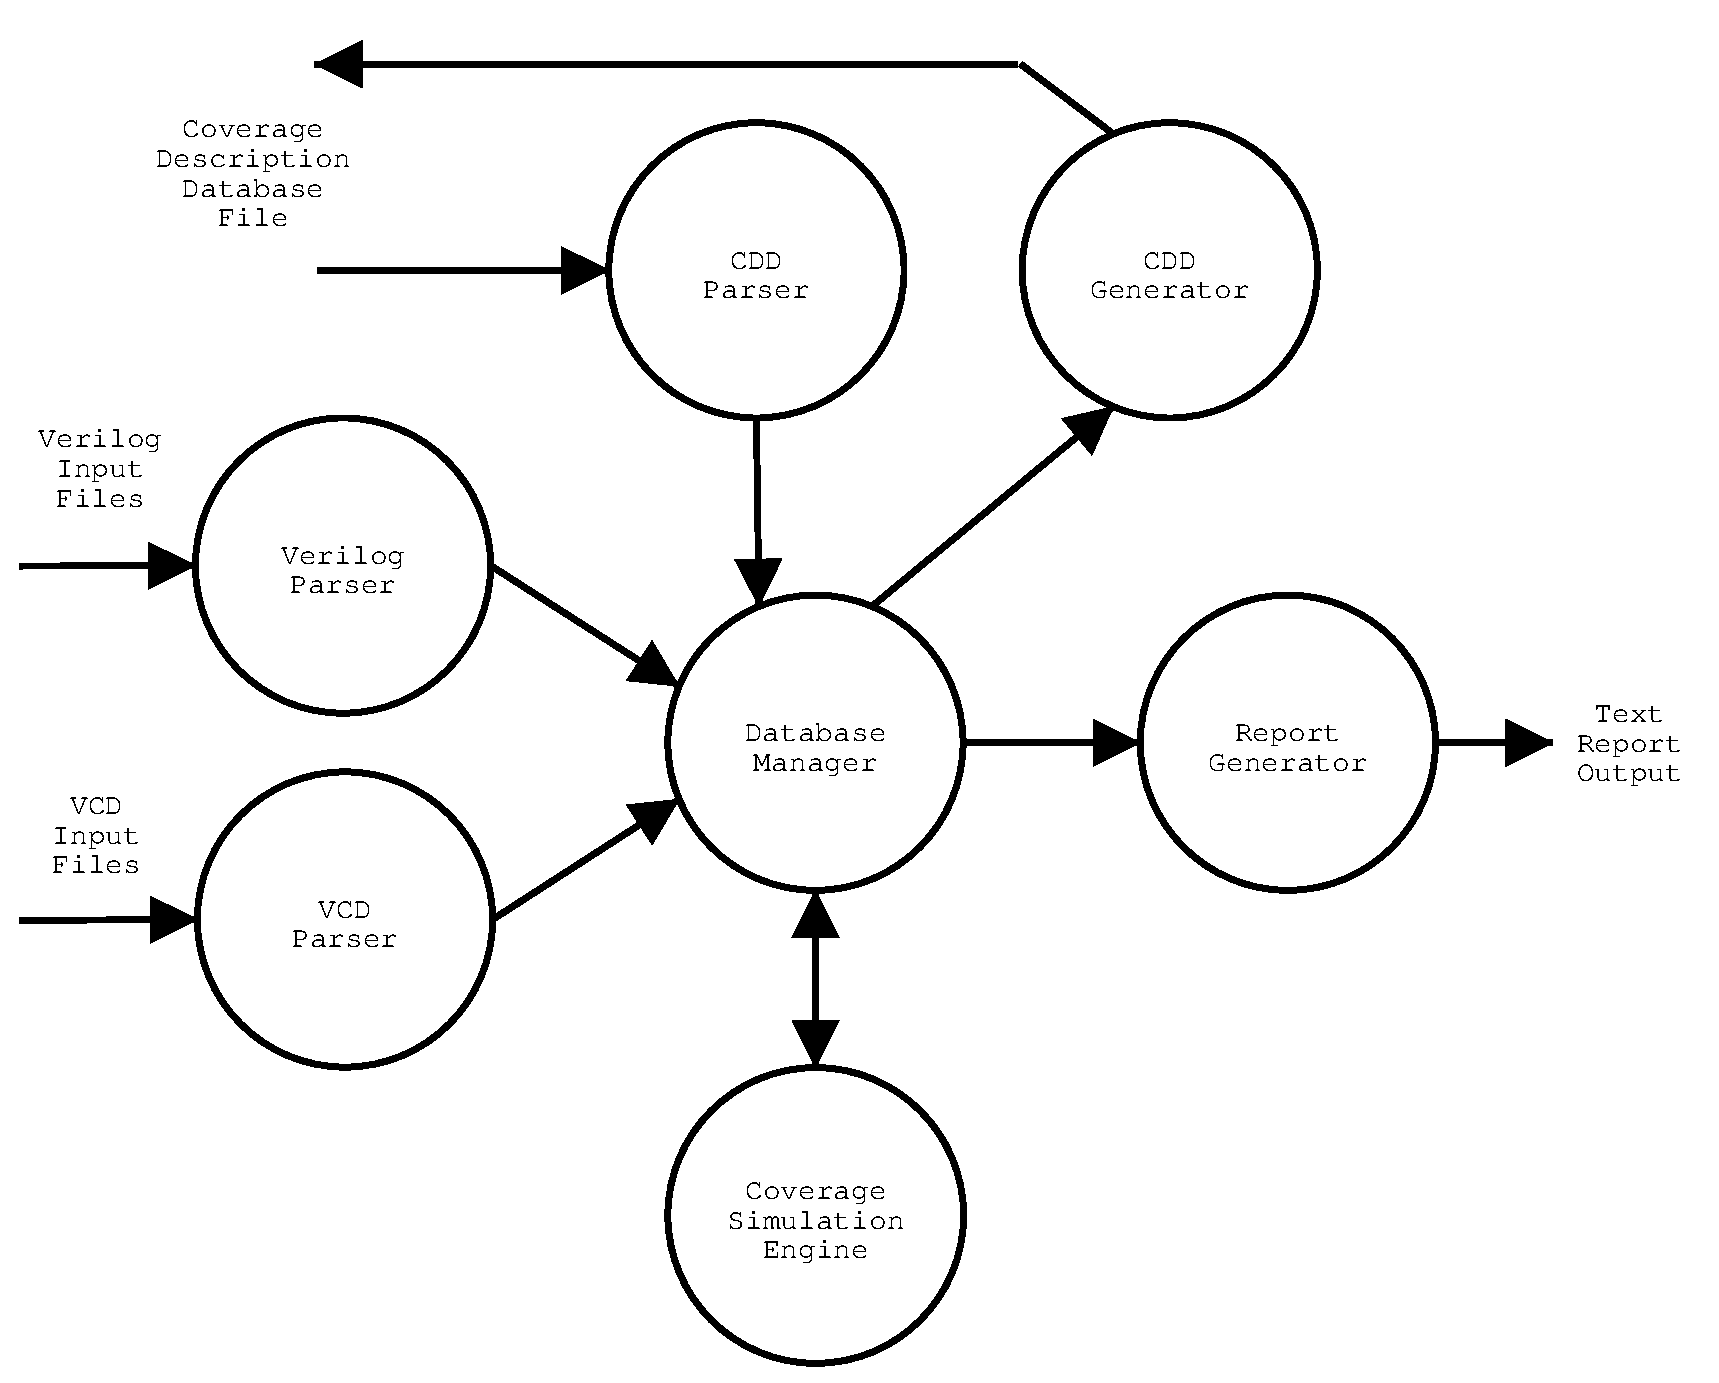
\includegraphics{big_picture}\caption{Figure 1. Data Flow Diagram}
\end{center}
\end{figure}
 \begin{Desc}
\item[]The following subsections describes each of these functions/nodes in greater detail.\end{Desc}
\begin{Desc}
\item[Section 5.2.1. Verilog Parser]\end{Desc}
\begin{Desc}
\item[]The Verilog parser used by Covered consists of a Flex lexical analyzer lexer.l and Bison parser parser.y . Both the lexer and parser where used from the Icarus Verilog project which can be accessed at:\end{Desc}
\begin{Desc}
\item[]{\tt http://icarus.com/eda/verilog/index.html}\end{Desc}
\begin{Desc}
\item[]Though most of the structure of both of these files maintain their original appearance from the Icarus project, most of the internal rule code has been removed and re-implemented to suite Covered's needs from the parser. The parser and lexer work together as most language parsers do with the lexer reading in tokens of information from the input files and passing these tokens for the parser to match with pre-existing language rules. The reason for taking both the lexer and parser from the Icarus project is that the Icarus project is well-used by the g\-EDA community for Verilog simulation and passes in regression the IV testsuite. This testsuite is available for download at:\end{Desc}
\begin{Desc}
\item[]{\tt http://ivtest.sourceforge.net}\end{Desc}
\begin{Desc}
\item[]Using the Verilog directory and file pathnames specified on the command-line, Covered generates a list of files to search for Verilog module names. The first module name that Covered attempts to find is the top-level module targetted for coverage. This module name is also specified on the command-line with the {\tt -t} option. The lexer reads in the file and finds the name specified after the Verilog keyword {\tt module}. If this module matches the top-level module name, the contents of the module are parsed. If the module name does not match the top-level module name, the lexer takes note of the found module and the filename in which it found the module and skips the body of the module until it encounters the {\tt endmodule} keyword. If there are any more modules specified in the given file, these are parsed in the same fashion. If the end of the file has been reached and no module has been found that is needed, the Verilog file is placed at the end of the file queue and the next file at the head of the queue is read in by the lexer.\end{Desc}
\begin{Desc}
\item[]If the top-level module contains module instantiations that also need to be tested for coverage, these module names are placed at the tail of the needed module queue. When the needed module queue is empty, all modules have been found and parsed, and the parsing phase of the procedure is considered complete and successful.\end{Desc}
\begin{Desc}
\item[]When the parser finds a match for one of its rules, an action is taken. This action is typically one of the following:\end{Desc}
\begin{Desc}
\item[]\begin{enumerate}
\item Create a new structure for data storage. \item Store a structure into one of the lists or trees for later retrieval. \item Manipulate a structure based on some information parsed. \item Display an error message due to finding code that is incorrect language structure. \end{enumerate}
\end{Desc}
\begin{Desc}
\item[]The Verilog parser only sends information to and gets information from the database manager. When parsing is complete, the database manager contains all of the information from the Verilog design which is stored in special containers which are organized by a group of trees and lists.\end{Desc}




\begin{Desc}
\item[Section 5.2.2. Database Manager]\end{Desc}
\begin{Desc}
\item[]The primary code of the database manager can be found in {\bf db.c}{\rm (p.\,\pageref{db_8c})} though the database management is distributed among several files. The database manager, as seen in the above diagram, is at the center of activity within the tool. All Verilog and VCD file information is stored in the database manager and all CDD output and report output is generated from it. The primary role of the database manager is to take the information from the Verilog, CDD and VCD parsers and populate two main global structures, an instance tree and a module list.\end{Desc}
\begin{Desc}
\item[]The instance tree root is pointed to by the global variable instance\_\-root. The file {\bf instance.c}{\rm (p.\,\pageref{instance_8c})} contains the functions that are used to add to, search, remove from and destroy that instance tree. The instance tree is composed of mod\_\-inst elements which are constructed to match the Verilog hierarchy of the DUT with the top-level DUT module at the top of the instance\_\-root tree. Each module instance element contains an instance name along with a pointer to a module element. During the parsing phase, several module instance elements may point to the same module element. After the parsing phase is completed an intermediate CDD file is generated in which each module instance is output in its entirety. Thus when the CDD is reread for scoring, merging or reporting each module instance is allocated its own module element (this is necessary to avoid simulation errors and to allow instance-based reports to be properly generated).\end{Desc}
\begin{Desc}
\item[]The module list is maintained by two pointers: mod\_\-head (points to head element of list) and mod\_\-tail (points to the tail element of list). New modules are always added to the tail of the list. Each module element in the list holds the name of the module, the file the module was taken from, and a set of lists containing all of the module's signals, expressions, statements, and parameters. All of the coverage information is stored in the signal and expression lists. For more detailed information on each of these types, see their corresponding code file in the detailed information section (signal = {\bf signal.c}{\rm (p.\,\pageref{signal_8c})}; expression = {\bf expr.c}{\rm (p.\,\pageref{expr_8c})}; statement = {\bf statement.c}{\rm (p.\,\pageref{statement_8c})}; parameter = {\bf param.c}{\rm (p.\,\pageref{param_8c})}). The module list is not necessary as far as keeping track of this module information (since the module instances point to these structures). Rather the list is maintained because information retrieval is sometimes much quicker than searching the module instance tree.\end{Desc}
\begin{Desc}
\item[]After the database manager has built these two structures (by getting information from the Verilog parser or the CDD file parser), other operations can be performed on these structures or information can be retrieved from them.\end{Desc}
\begin{Desc}
\item[]Each of Covered's commands (score, merge, report) contains a series of phases for moving data. The following subsections describe the database manager's role in each of these phases.\end{Desc}
\begin{Desc}
\item[Section 5.2.2.1. Score Command Phases]\end{Desc}
\begin{Desc}
\item[]The score command is the initial Covered command that turns Verilog and VCD input into a populated CDD database file. The score command contains five phases as described below.\end{Desc}
\begin{Desc}
\item[]\begin{enumerate}
\item Parsing Phase \begin{itemize}
\item Verilog files are read in by Covered and its information stored into the instance tree and module list structures. \end{itemize}
\item CDD Generation Phase \begin{itemize}
\item Instance tree structure is initially written as an unpopulated CDD file. \end{itemize}
\item CDD Load Phase \begin{itemize}
\item Unpopulated CDD file read and information restored into instance tree and module list structures with each module instance receiving its own module element. \end{itemize}
\item VCD Load and Simulation Phase \begin{itemize}
\item VCD file read and coverage design resimulated based on VCD contents. During simulation coverage information is compiled and stored into proper signal and expression structures. \end{itemize}
\item CDD Final Output Phase \begin{itemize}
\item Instance tree structure is rewritten as a populated CDD file. \end{itemize}
\end{enumerate}
\end{Desc}
\begin{Desc}
\item[]After all five phases of the score command have been completed, the resulting CDD file is ready for merging or reporting. All phases of the score command can be found in the {\bf score.c}{\rm (p.\,\pageref{score_8c})} and {\bf parse.c}{\rm (p.\,\pageref{parse_8c})} source files.\end{Desc}
\begin{Desc}
\item[]It is important to note that after the first two phases have been completed, the resulting CDD file, though it doesn't contain any coverage information, contains all of the design information necessary for simulation. Therefore, if multiple VCD files are needed to be scored, phases 1 and 2 can be performed once, the unpopulated files can be manually copied by the user and renamed, and phases 3, 4 and 5 can be run once for each VCD file. This saves the time of having to perform phases 1 and 2 for each VCD simulation run.\end{Desc}
\begin{Desc}
\item[Section 5.2.2.2. Merge Command Phases]\end{Desc}
\begin{Desc}
\item[]The merge command is useful for combining the coverage information from two populated CDD files into one populated CDD file. The resulting CDD file is the union of the two merged CDD files. The merge command contains only three phases as described below.\end{Desc}
\begin{Desc}
\item[]\begin{enumerate}
\item CDD Load Phase \begin{itemize}
\item Reads in first CDD file and stores it into instance tree and module list structures. \end{itemize}
\item CDD Merge Phase \begin{itemize}
\item Reads in second CDD file, merging its contents into the existing instance tree and module list structures. All structures now contain merged data. \end{itemize}
\item CDD Final Output Phase \begin{itemize}
\item Outputs contents of instance tree structure to CDD file. \end{itemize}
\end{enumerate}
\end{Desc}
\begin{Desc}
\item[]After all three phases have been completed, the resulting CDD file is a union of the two input CDD files but remains in the exact same format as the CDD file read in by phase 1 of the merge. All phases of the merge command can be found in the {\bf merge.c}{\rm (p.\,\pageref{merge_8c})} source file.\end{Desc}
\begin{Desc}
\item[Section 5.2.2.3. Report Command Phases]\end{Desc}
\begin{Desc}
\item[]The report command is responsible for converting the cryptic CDD coverage file into human readable output to describe summary and/or verbose output. The report command is composed of three phases as described below.\end{Desc}
\begin{Desc}
\item[]\begin{enumerate}
\item CDD Load Phase \begin{itemize}
\item Input CDD file is loaded into instance tree and module list structures. \end{itemize}
\item Summary Statistical Gathering Phase \begin{itemize}
\item Summary statistics are calculated and stored for each metric. \end{itemize}
\item Report Output Phase \begin{itemize}
\item Summary, Detail and/or Verbose report is output to standard output or specified file. \end{itemize}
\end{enumerate}
\end{Desc}
\begin{Desc}
\item[]The report command is the only command whose output is not a CDD file. The report command treats the input CDD file as read-only and does not alter the files contents. All phases of the report command can be found in the {\bf report.c}{\rm (p.\,\pageref{report_8c})} source file.\end{Desc}




\begin{Desc}
\item[Section 5.2.3. CDD Parser]\end{Desc}
\begin{Desc}
\item[]The Coverage Description Database file, or CDD as it is referred to in this documentation, is a generalized description of a Verilog design that contains coverage-specific information as it pertains to that design. CDD files are in ASCII text format. The reasons for having this file format are three-fold.\end{Desc}
\begin{Desc}
\item[]\begin{enumerate}
\item Allow a way to store information about a particular design in a way that is compact and concise. It is understood that a CDD file may exist for an indeterminant amount of time so it is important that the file size be as small as possible while still carrying enough information to generate useful coverage reports. \item Create a standardized output format that is easy to parse (can be done with the sscanf utility in a straight-forward way) not requiring the use and overhead of another lexer and parser. The standardization of the file format allows several CDDs to be easily merged and output in the same format. \item Create a format that is flexible enough to add new constructs as needed to support the growing Verilog language while not making it more difficult to parse. \end{enumerate}
\end{Desc}
\begin{Desc}
\item[]The generic output format for the CDD file is as follows:\end{Desc}
\begin{Desc}
\item[]{\tt }  {\tt } \end{Desc}
\begin{Desc}
\item[]If a new construct needs to be added to the tool, one merely needs to select a unique ID for that construct and come up with a format for displaying the information for that construct so that it is separated by spaces or commas and contains only one ENDLINE character at the end of the line. Blank lines or comments are allowed within the file. The current constructs that are output to a CDD file by Covered are listed below along with their unique ID.\end{Desc}
\begin{Desc}
\item[]\begin{itemize}
\item signal (1; {\bf signal.c}{\rm (p.\,\pageref{signal_8c})}) \item expression (2; {\bf expr.c}{\rm (p.\,\pageref{expr_8c})}) \item module (3; {\bf module.c}{\rm (p.\,\pageref{module_8c})}) \item statement (4; {\bf statement.c}{\rm (p.\,\pageref{statement_8c})}) \item info (5; {\bf info.c}{\rm (p.\,\pageref{info_8c})}) \end{itemize}
\end{Desc}
\begin{Desc}
\item[]The information format for each construct is listed with the description of the construct in the {\bf Section 6.  Coverage Development Reference}{\rm (p.\,\pageref{page_code_details})} section.\end{Desc}
\begin{Desc}
\item[]Each line of the CDD file is read into memory by the CDD parser and the first value of the line (the unique construct ID) is used to call the {\tt db\_\-read} function of the associated construct. The construct then takes the initiative of decoding the rest of the line and storing its contents into the same set of lists and trees that the Verilog parser stores its information into. The end result of parsing in the CDD file is the same as parsing in a design by the Verilog parser. Once into memory, the information can be merged, simulated, or computed on by the report generator.\end{Desc}




\begin{Desc}
\item[Section 5.2.4. CDD Generator]\end{Desc}
\begin{Desc}
\item[]The CDD generator is actually distributed among the various constructs that make up the CDD file. The main {\tt db\_\-write} function located in {\bf db.c}{\rm (p.\,\pageref{db_8c})} calls each of the construct's {\tt db\_\-write} functions which, in turn, output their information to the CDD file in their own format. After each of the stored constructs have written their information to the CDD file, it is closed by the {\tt db\_\-write} function. The end result is a CDD file that is in the same format as the CDD file that was read in by the CDD parser.\end{Desc}




\begin{Desc}
\item[Section 5.2.5. VCD Parser]\end{Desc}
\begin{Desc}
\item[]After a design or CDD has been stored internally into the database manager's memory, that memory may be merged with the data stored in another CDD, used to generate a report, or simulated with the use of the input from a VCD file that was created from the design loaded into the database manager's memory. In the last scenario, the VCD parser is invoked to read in the contents of the specified VCD dumpfile. The VCD parser can read in any VCD file that is output according to the VCD format. The format of VCD can be found at:\end{Desc}
\begin{Desc}
\item[]{\tt http://www-ee.eng.hawaii.edu/$\sim$msmith/ASICs/HTML/Verilog/LRM/HTML/15/ch15.2.htm\#pgf\-Id=250}\end{Desc}
\begin{Desc}
\item[]The VCD parser is written using the fscanf and sscanf utilities. Due to the ambiguity of the VCD file format, it was decided to write the parser using these utilities instead of the standard flex and bison. In addition to ease of code writing, the fscanf and sscanf readers are more efficient than the alternative. All VCD file parsing is contained in the {\bf vcd.c}{\rm (p.\,\pageref{vcd_8c})} source file.\end{Desc}




\begin{Desc}
\item[Section 5.2.6. Coverage Simulation Engine]\end{Desc}
\begin{Desc}
\item[]Because Covered determines coverage for a simulation without participating in the actual Verilog simulation (this is because Covered does not \char`\"{}annotate\char`\"{} the design prior to compilation/simulation), a \char`\"{}resimulation\char`\"{} of the original is necessary using the VCD file as the means of data input. The \char`\"{}resimulation\char`\"{} can be performed much quicker than the original simulation because many details that the actual Verilog simulator needs to handle and account for can be ignored by Covered. Intermediate calculations are not performed in a given timestep, since such \char`\"{}glitches\char`\"{} can generate bad/misleading coverage information, only the last value of a given signal is used in calculations. These optimizations/shortcuts can make resimulation quick but cannot be entirely eliminated. Though it is possible to calculate toggle coverage using only the VCD file and no simulation, metrics like line, combinational logic and FSM coverage require simulation data.\end{Desc}
\begin{Desc}
\item[]The simulation engine in Covered is closely tied to the VCD parser. When the VCD parser is parsing the value change portion of the VCD file, value changes are recorded by associating a value to the signal specified by the VCD symbol. The symbol and value are stored in a tree structure for quick lookup. Entries in this table are sorted/searched by symbol string value. When a timestep is encountered in the VCD table, the simulation engine is invoked for that timestep in which it carries out two operations.\end{Desc}
\begin{Desc}
\item[Section 5.2.6.1. Symbol Table Transfer Operation]\end{Desc}
\begin{Desc}
\item[]The first operation of the simulation engine is to transfer the information stored in the symbol/value table to the associated signals. This operation is known as symbol table transfer and is performed by the function symtable\_\-assign located in the {\bf symtable.c}{\rm (p.\,\pageref{symtable_8c})} source file. In this operation, the tree that contains the current timestep symbols/values (timestep\_\-tab) is traversed, assigning the stored value to the signal structure that is associated with the stored symbol. When this operation occurs, toggle coverage information is obtained glitch-free and all statements containing those signals are flagged as being modified and placed in a special queue known as the pre-simulation queue (please see {\bf sim.c}{\rm (p.\,\pageref{sim_8c})} for more details). After all entries in the timestep\_\-tab symbol tree have been traversed, the entire tree is deallocated from memory, ready for the next timestep information.\end{Desc}
\begin{Desc}
\item[Section 5.2.6.2. Statement Simulation Operation]\end{Desc}
\begin{Desc}
\item[]The second operation of the simulation engine is the actual simulation itself. The source code for the simulation engine is located in {\bf sim.c}{\rm (p.\,\pageref{sim_8c})}. During the statement simulation operation, the statement at the head of the pre-simulation queue is evaluated (combinational and line coverage metrics are obtained at this time) and statements within its statement tree (a.k.a., statement block) traversed and executed accordingly. When a statement tree has completed it is removed from the pre-simulation queue and the next statement in the pre-simulation queue is executed. If a statement tree hits a delay or wait event, the statement pointer in the pre-simulation queue is updated to point to the current statement and the next statement in the pre-simulation queue is simulated. This process continues until all statements in the pre-simulation queue have been simulated.\end{Desc}




\begin{Desc}
\item[Section 5.2.7. Report Generator]\end{Desc}
\begin{Desc}
\item[]The report generator is rooted in the file {\bf report.c}{\rm (p.\,\pageref{report_8c})}; however, the actual job of generating a report is distributed among five source files:\end{Desc}
\begin{Desc}
\item[]\begin{enumerate}
\item {\bf line.c}{\rm (p.\,\pageref{line_8c})} (Line coverage output) \item {\bf toggle.c}{\rm (p.\,\pageref{toggle_8c})} (Toggle coverage output) \item {\bf comb.c}{\rm (p.\,\pageref{comb_8c})} (Combinational logic coverage output) \item {\bf codegen.c}{\rm (p.\,\pageref{codegen_8c})} (Reconstructs Verilog code from expression tree information) \item {\bf fsm.c}{\rm (p.\,\pageref{fsm_8c})} (Finite State Machine coverage output) \end{enumerate}
\end{Desc}
\begin{Desc}
\item[]Once the CDD has been loaded into the instance\_\-root module instance tree, the report generator calls each metric's statistical generator. Each statistical generator traverses through the various signal/expression/statement lists gaining summary coverage information for each module/instance. This information is stored in the statistic structure associated with each module instance in the design. When outputting occurs, the statistic structure is used to generate the summary coverage data. The source file for handling statistical structures can be found in {\bf stat.c}{\rm (p.\,\pageref{stat_8c})}.\end{Desc}
\begin{Desc}
\item[]The second phase of the report generator is the output of information. In all cases, summary information is output to the report (as mentioned above). If the user has specified summary information only, report outputting is complete once all user specified metrics have been output in summary form. If the user has specified detailed or verbose reports, the report generator must generate this information to the report. Each metric accomplishes this output in different ways according to its metric type. Please refer to the metric report file for more information in what is necessary to generate the detailed/verbose report.\end{Desc}




\begin{Desc}
\item[Go To Section...]\begin{itemize}
\item {\bf Section 1.  Introduction}{\rm (p.\,\pageref{page_intro})}\item {\bf Section 2.  Project Plan}{\rm (p.\,\pageref{page_project_plan})}\item {\bf Section 3.  Coding Style Guidelines}{\rm (p.\,\pageref{page_code_style})}\item {\bf Section 4.  Development Tools}{\rm (p.\,\pageref{page_tools})}\item {\bf Section 6.  Coverage Development Reference}{\rm (p.\,\pageref{page_code_details})}\item {\bf Section 7.  Test and Checkout Procedure}{\rm (p.\,\pageref{page_testing})}\item {\bf Section 8.  Debugging}{\rm (p.\,\pageref{page_debugging})}\item {\bf Section 9.  Odds and Ends Information}{\rm (p.\,\pageref{page_misc})} \end{itemize}
\end{Desc}
